%%%%%%%%%%%%%%%%%%%%%%%%%%%%%%%%%%%%%%%%%
% Short Sectioned Assignment
% LaTeX Template
% Version 1.0 (5/5/12)
%
% This template has been downloaded from:
% http://www.LaTeXTemplates.com
%
% Original author:
% Frits Wenneker (http://www.howtotex.com)
%
% License:
% CC BY-NC-SA 3.0 (http://creativecommons.org/licenses/by-nc-sa/3.0/)
%
%%%%%%%%%%%%%%%%%%%%%%%%%%%%%%%%%%%%%%%%%

%----------------------------------------------------------------------------------------
%	PACKAGES AND OTHER DOCUMENT CONFIGURATIONS
%----------------------------------------------------------------------------------------

\documentclass[paper=a4, fontsize=11pt]{scrartcl} % A4 paper and 11pt font size

\usepackage[T1]{fontenc} % Use 8-bit encoding that has 256 glyphs
\usepackage[ngerman]{babel}
\usepackage{fourier} % Use the Adobe Utopia font for the document - comment this line to return to the LaTeX default
\usepackage{amsmath,amsfonts,amsthm} % Math packages
\usepackage{graphicx}
\usepackage[utf8]{inputenc}
\usepackage{listings}
\usepackage[section]{placeins}
\usepackage{lipsum} % Used for inserting dummy 'Lorem ipsum' text into the template
\usepackage{float}
\usepackage{multicol}
\usepackage{algpseudocode}
\usepackage{algorithm}% http://ctan.org/pkg/algorithms

% Algorithmic modifications
\makeatletter
\newcommand{\ALOOP}[1]{\ALC@it\algorithmicloop\ #1%
  \begin{ALC@loop}}
\newcommand{\ENDALOOP}{\end{ALC@loop}\ALC@it\algorithmicendloop}
\renewcommand{\algorithmicrequire}{\textbf{Input:}}
\renewcommand{\algorithmicensure}{\textbf{Output:}}
\newcommand{\algorithmicbreak}{\textbf{break}}
\newcommand{\BREAK}{\STATE \algorithmicbreak}
\makeatother

\usepackage{sectsty} % Allows customizing section commands
\allsectionsfont{\centering \normalfont\scshape} % Make all sections centered, the default font and small caps

\usepackage{fancyhdr} % Custom headers and footers
\pagestyle{fancyplain} % Makes all pages in the document conform to the custom headers and footers
\fancyhead{} % No page header - if you want one, create it in the same way as the footers below
\fancyfoot[L]{} % Empty left footer
\fancyfoot[C]{} % Empty center footer
\fancyfoot[R]{\thepage} % Page numbering for right footer
\renewcommand{\headrulewidth}{0pt} % Remove header underlines
\renewcommand{\footrulewidth}{0pt} % Remove footer underlines
\setlength{\headheight}{13.6pt} % Customize the height of the header

\numberwithin{equation}{section} % Number equations within sections (i.e. 1.1, 1.2, 2.1, 2.2 instead of 1, 2, 3, 4)
\numberwithin{figure}{section} % Number figures within sections (i.e. 1.1, 1.2, 2.1, 2.2 instead of 1, 2, 3, 4)
\numberwithin{table}{section} % Number tables within sections (i.e. 1.1, 1.2, 2.1, 2.2 instead of 1, 2, 3, 4)

\setlength\parindent{0pt} % Removes all indentation from paragraphs - comment this line for an assignment with lots of text

\DeclareMathOperator*{\argmin}{arg\,min}

%----------------------------------------------------------------------------------------
%	TITLE SECTION
%----------------------------------------------------------------------------------------

\newcommand{\horrule}[1]{\rule{\linewidth}{#1}} % Create horizontal rule command with 1 argument of height

\title{
\normalfont \normalsize
\textsc{Karlsruher Insitut für Technologie} \\ [25pt] % Your university, school and/or department name(s)
\horrule{0.5pt} \\[0.4cm] % Thin top horizontal rule
\huge Softwaretechnik II\\ Zusammenfassung WS17/18 % The assignment title
\horrule{2pt} \\[0.5cm] % Thick bottom horizontal rule
}

\author{Manuel Lang} % Your name

\date{\normalsize\today} % Today's date or a custom date

\begin{document}

\maketitle % Print the title
%\newpage
%\tableofcontents
%\newpage

\section{Vorgehensmodelle}

Vorteile strukturierter Vorgehensmodelle
\begin{itemize}
  \item Reproduzierbarkeit (Erfahrungen für ähnliche Projekte)
  \item Skalierbarkeit (größere Komplexität schneller)
  \item Wiederverwendbarkeit (Code)
  \item Risikominimierung (Entiwcklung nach Plan)
\end{itemize}

Modelle
\begin{itemize}
  \item Softwareentwicklung liefert nicht nur Code, sondern auch Deployment-Deskriptoren (Zusazudokumente), ursprüngliche Anforderungen (Code -> Anforderungen funktioniert nicht), welche Produkte wann und wo?
  \item Wasserfall-Modell\\
  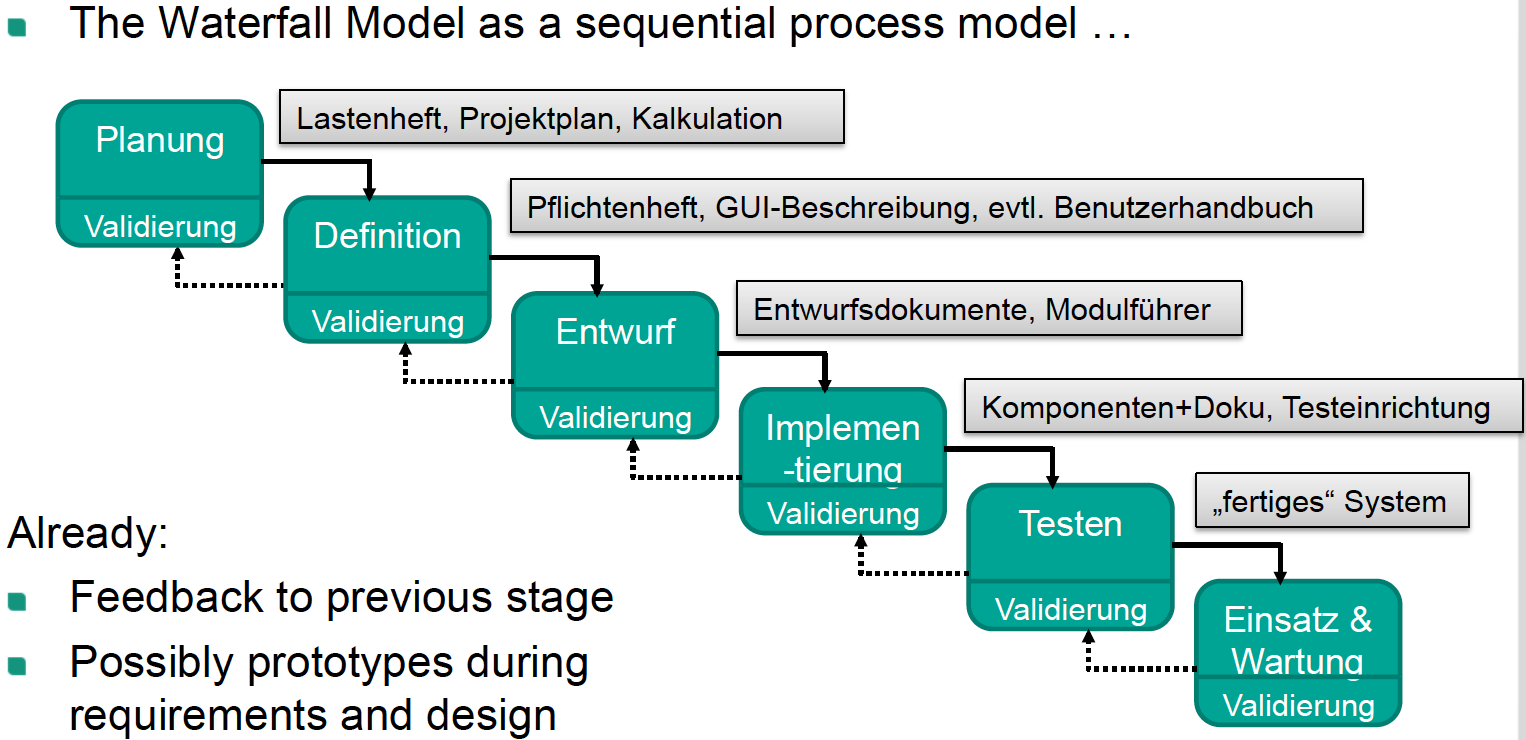
\includegraphics[width=\linewidth]{imgs/wasserfall}
  \begin{itemize}
    \item Erstes Modell zur Definition der verschiedenen Phasen
    \item überhaupt machbar?
    \item Welche Stakeholder?
    \item Lastenheft/Pflichtenheft
    \item etc.
    \item Problem: sehr steife Reihenfolge, klingt logisch, aber Phasenübergang ist in Realität unklar
    \item Feedbackzyklen nötig, aber Unterscheidbarkeit der Phasen trotzdem schwierig
    \item Zu langes Vorplanen (Airbus 10 Jahre?!) sehr schwierig, Was kann in der Zwischenzeit passieren? Niemand weiß das, daher kann Wasserfall langfristig nicht geplant werden (lange Planbarkeit nur sehr selten gegeben)
  \end{itemize}
  \item V-Modell\\
  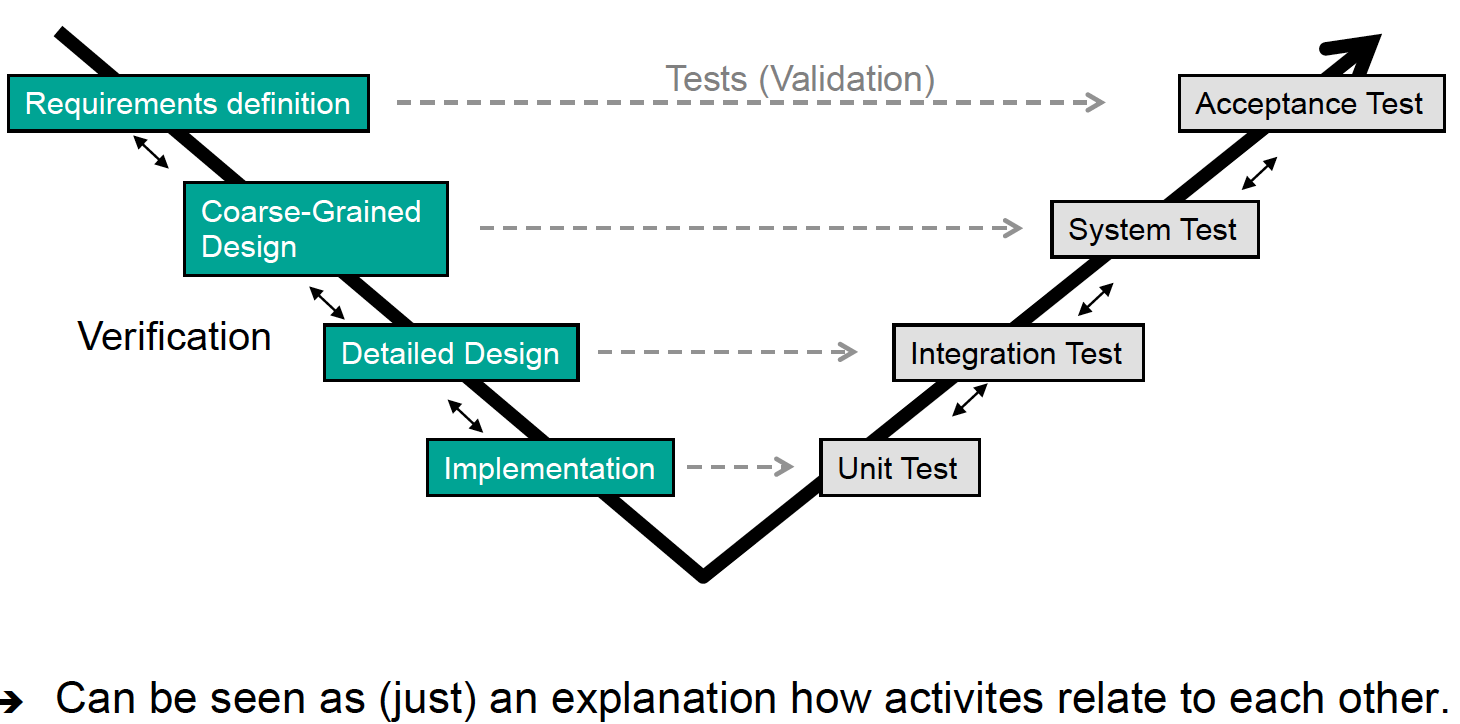
\includegraphics[width=\linewidth]{imgs/vmodell}
  \begin{itemize}
    \item sieht ähnlich aus wie Wasserfall
    \item besagt welche Artefakte man hat + erklärt Zusammenhänge zwischen Dokumenten
    \item überprüft bspw. Zusammenhang zwischen Implementierung und Design (Verifikation, zeigt Abwesenheit von Fehlern, All-Quantor funktioniert immer)
    \item Z.B. mehrere Module zusammen testen (Validierung, nicht Verifikation, Existenz-Quantor, Test-Fall der funktioniert)
    \item Hauptbotschaft: kein notwendiger Wasserfall: Artefakte + Zusammenhänge (Validierung + Verifikation)
  \end{itemize}
  \item 6 grundlegende Phasen in jedem SE-Projekt
  \begin{itemize}
    \item Planung
    \item Definition
    \item Design/Entwurf
    \item Implementierung
    \item Testen
    \item Betrieb
    \item Wartung
  \end{itemize}
  \item 3 Dinge über die ein SE-Modell Aussagen trifft
  \begin{itemize}
    \item Welche Rollen?
    \item Welche Aktivitäten?
    \item Welche Produkte?
  \end{itemize}
  \item Probleme des Wasserfall-Modells
  \begin{itemize}
    \item Sehr lange Zeiträume
    \item inflexibel (schlecht auf Änderungen reagierbar)
  \end{itemize}
  \item Alternativen?
  \begin{itemize}
    \item Inkrementeller Ansatz (nicht zwangsweise flexibel bei geänderten Anforderungen, sondern große Komplexität: mehrere Zyklen für kleinere Teilprojekte), viele kleine kürzere Wasserfälle
    \item Evolutionär: Bei "Fertigstellung" zurückspringen z.B. in Planungsphase, in der Praxis fast immer da z.B. langzeitig Änderungsbedarf auftritt
    \item Gesamtsystem wird nach und nach gebaut
    \item Integrationstests, immer neue Inkremente für Kunden für schnelles Feedback
    \item Konzepte der agilen Entwicklung schon älter
  \end{itemize}
  \item Spiralmodell
  \begin{itemize}
    \item Idee: 4 Quadranten, Zielfestlegung, Bewertung, Validierung, Planung, immer im Kreis um Irrglauben Software ist irgendwann fertig auszuräumen
    \item Nicht inkrementell, sondern evolutionär
  \end{itemize}
  \item UP (Unified Process)\\
  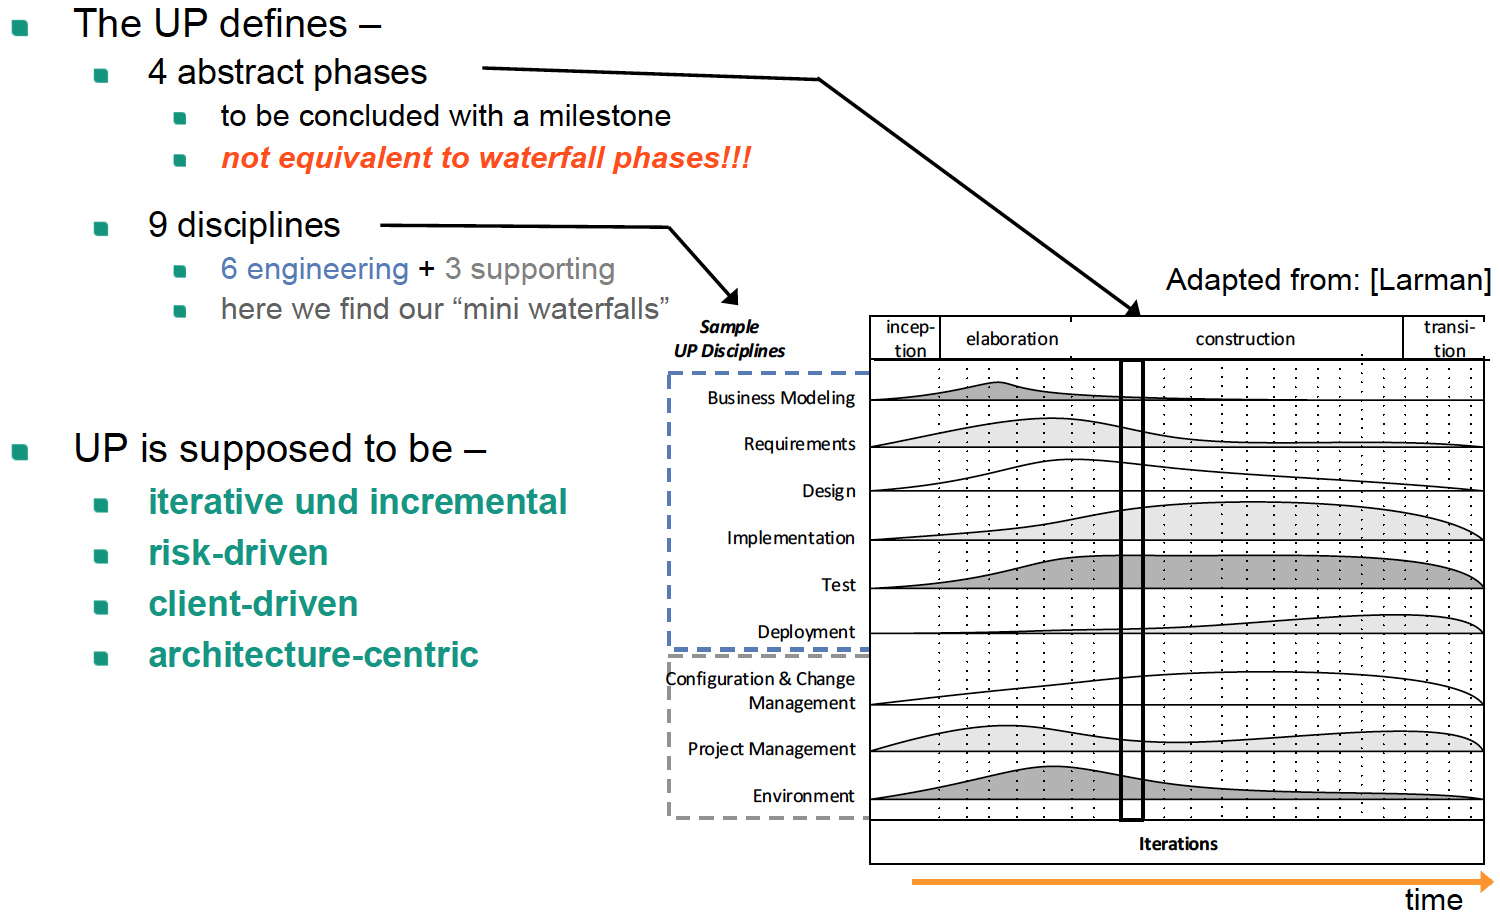
\includegraphics[width=\linewidth]{imgs/up}
  \begin{itemize}
    \item zuerst UML: vereinheitlichte Notation, z.B. Symbole für Widerstände und Transistoren, Industriestandard
    \item Folge: vereinheitlichte Prozesse, also UP, aber komplett verschieden zu UML (einheitlich), aber es gibt nicht den einen richtigen Software-Prozess, hängt von vielen verschiedenen Faktoren ab (z.B. eingebettete Software), also Rahmenwerk für Prozesse
    \item Verschiedene Phasen: Inception, Elaboration, Konstruktion, Transition über Zeitachse
    \item Verschiedene Disziplinen wie früher Phasen, auch mit Deployment, insgesamt moderner, andere Disziplinen wie Änderungsmanagement, Projektmanagement, Environment (Entwicklungsumgebung) = Aufrechterhalten der Produktivumgebung + Zusammenspiel der Komponenten + Patches
    \item iterativ und inkrementell (streng nicht dasselbe, iterativ mehrere Schleifen durch Prozess, inkrementell heißt neues Teil), quasi Synonyme
    \item Risiko-getrieben, sehr früh auf Risiken reagierbar
    \item Client-driven: Was will der Auftraggeber?
    \item Architektur-zentriert: zentrales Dokument wovon andere Aktivitäten abhängen
    \begin{itemize}
      \item Inception (Anfangsphase): Scope, Business cases?, machbar?, auf Markt?, Kostenschätzung (schwierig so früh, also sehr grob)
      \item Elaboration (Ausarbeitung): Besonders risikobehaftete Teile werden zuerst betrachtet, Anforderungen verstehen, Übergang in Konstruktionsphase, klappt gut mit sehr erfahreren Entwicklern die Abstraktionsebenen einfach wechseln können, sonst problematisch
      \item Konstruktionsphase
      \item Übergabephase (Test, Deployment)
    \end{itemize}
    \item Disziplinen
    \begin{itemize}
      \item Business Modelling: Technische Konzepte
      \item Anforderungen: Anforderungsanalyse, Dokumentation
      \item Entwurf: Lösungsorientiert, aber kleine klare Grenze zu Anforderungen, nicht nur zeitlich sondern auch konzeptionell überlappend
      \item keine klaren Definitionen!
    \end{itemize}
  \end{itemize}
  \item Rational Unified Process (RUP)
  \begin{itemize}
    \item 6 best practices (sehr generelle Aussagen): iterativ entwickeln, Anforderungen verwalten, Komponenten verwenden, Software grafisch visualisieren, Softwarequalität prüfen, Änderungen unter Kontrolle haben
    \item Was konkret in welcher Phase wurde definiert, konkrete Aufgaben, konkret welche Artefakte
    \item verschiedene Rollen für verschiedene Disziplinen definiert, Anpassungen für konkrete Projekte
    \item prinzipiell genauere Ausarbeitung des UP
  \end{itemize}
  \item Rollen
  \begin{itemize}
    \item Verantwortung abgekoppelt von Person, Reussner Prof. + Vater + Vorstand
    \item eine Person kann mehrere Rollen annehmen
    \item kann aber zu viel Verschnitt führen (viele stehen rum und einer arbeitet, d.h. Gefahr, dass jeder in seiner Rolle bleibt, aber nicht flexibel ist)
  \end{itemize}
  \item Zusammenfassung
  \begin{itemize}
    \item iterativ
    \item UP: Phasen + Disziplinen
    \item RUP: Aktivitäten, Artefakte, Rollen, Rahmenwerk für Projekte
    \item nicht ein gültiger Prozess
  \end{itemize}
  \item Agile Methoden
  \begin{itemize}
    \item kein Allheilmittel
    \item Manifest für agile Softwareentwicklung: Individuals/Interactions > Prozesse, Software > Doku, Kundenzufriedenheit > Vertragsverhandlungen, Flexibilität > Plan folgen
    \item Ist das tatsächlich nötig oder wird Feindbild aufgebaut? Leichter wogegen als wie besser, daher Kritik dass eh niemand so stur ist
    \item Quintessenz: nicht beliebig planbar (Änderungen kommen immer), kontinuierliche Beobachtungen und schnelles Feedback (bau ich was Kunde will? ist Qualität gut?)
  \end{itemize}
  \item Extreme Programming (XP)
  \begin{itemize}
    \item Programmieren = zentral, alles andere außen rum
    \item innen Entwickler: einfache Entwürfe für aktuelle Anforderung, Realisierung mit Pair Programming (verdoppelt Kosten, nicht immer gerechtfertigt, verbessert Qualität auch nicht besser als andere Review-Formen), testgetriebene Entwicklung (immer testbare Software + i.d.R. besser testbare Schnittstellen), Refactoring (Anpassen des Entwurfs für weitere Anforderungen)
    \item außenrum Team: Continuous Integration (keine großen Aufwände bei Builds), Collective Ownership (jeder für alles verantwortlich, kann aber auch fehlschlagen, daher Gesamtprojektverantwortung), Coding Standard
    \item äußerster Kreis: kleine Releases für schnelles Feedback, Kunden testen mit, Planungsspiele (Aufteilen der Inkremente)
    \item Kritik: ad-hoc Prozess, schwer replizierbar, schlechte Doku, nicht wiederverwendbare Software, Kunden müssen eingebunden werden (will Kunde das?), vieles nicht wissenschaftlich validiert (z.B. Pair Programming), TDD kann problematisch sein
    \item endet in Praxis oft in Code \& Fix
  \end{itemize}
  \item Scrum
  \begin{itemize}
    \item Rahmenwerk mit notwendigen Anpassungen, aber ziemlich elaboriert
    \item Name von Rugby
    \item Product Owner verantwortlich für zu realisierende User Stories und landen als Sammlung in Product Backlog
    \item Inkremente (Sprints): Planning Meeting Product Backlog in Sprint Backlog, Dauer 2-4 Wochen aber konstant
    \item Daily Scrum: täglicher Projektfortschritt, Burn Down Chart (Liste der offenen TODOs abgearbeitet)
    \item Scrum Master trainiert das Team, sorgt dafür, dass sich Entwickler auf das Entwickeln konzentrieren können (also eine stabile Arbeitsumgebung)
    \item Sprint Review Meeting: Wie war die Qualität?
    \item Retroperspective Meeting (Ende vom Projekt): Was hätte man besser machen können? Lehren?
    \item Rollen (pig rolls treiben voran - essentiell): Product Owner (Kundenstellvertreter, vergleichbar mit Architekt), Scrum Master (Hindernisse ausgeräumt, verantwortlich dass Vorgang läuft, damit Entwickler sich auf Rolle konzentrieren können), Team (selbstorganisiert, kümmert sich um Produkt, keine Hierarchie wie bei XP, etwa 7 Leute meist), (chicken rolls - nicht essentiell) Stakeholder, Manager, etc., dürfen Pigs nicht sagen wie sie ihre Arbeit machen
    \item oft TDD
    \item Product Backlog: Sammlung aller Anforderungen, dynamisches Dokument, Priorisierung der Features (z.B. wie stark wird Architektur beeinflusst, wie stark sind Risiken)
    \item Projektplanung: nach jedem Sprint kann etwas ausgeliefert werden, damit schnell Feedback erlangt werden kann, Planung auf 3 Ebenen: Release, Sprint, Arbeitstag
    \item Sprint Backlog: zerbröselter abstrakter Product Backlog für aktuellen Sprint in konkrete Arbeitsaufgabgen, Absprache mit Kunde vlt. nötig, Kategorien: to do, in progress, finished, aber Definition of done?, Sprint Backlog in Product Backlog ist nicht vorgesehen, aber möglich
    \item Sprint Backlog füllen: User Stories vom Product Backlog mit Product Owner und Team Membern diskutiert, oder vielleicht erst Prototyp nötig? Aktivität sollte nicht länger als 2 Tage sein, damit guter Überblick möglich, Abschätzen in Personenstunden, keine Puffer sondern präzise schätzen bspw. durch Time-Box (z.B. 2 Tage nehmen und unter Umständen neu planen)
    \item Wie viel ist genug? Geplant wird weniger, bspw.85\% der Kapazität und zusätzlich etwa 25\% Abzug (Meetings, Urlaub, Krankheit)
    \item Burn Down Chart (Abarbeitung des Product Backlogs über verschiedene Sprints, Infos über Arbeitsgeschwindigkeit zur besseren Planung)
    \item Kritische Bewertung
    \begin{itemize}
      \item Personen/Rollen: Entwickler müssen nahe beisammen sein, kann nur gut klappen wenn sich alle Leute dran halten (benötigt viel Disziplin), effiziente Kommunikation ist wichtig, klappt aber nicht mit vielen Leuten
      \item Artefakte: keine Dokumentation vorgesehen (nur wenn explizit geplant), Code + Testfälle (reicht oft nicht)
      \item Dokumente: -
      \item Aktivitäten: keine Phase zu Architekturentwurf (in Praxis oft Sprint 0 - Architektur)
      \item Skalierbarkeit: sehr schlecht, weil nur für wenig Leute vorgesehen
      \item Architektur: nicht per se vorgesehen
      \item Qualitäts-kritische Software: per se kein Grund wieso nicht agil, aber sehr gute Qualitätssicherung für Sonderfälle sehr wichtig (z.B. Abschaltung Atomkraftwerk), die normalerweise nicht Teil von Scrum sind
      \item große Projekte: Brook's Law (spätes Hinzufügen von Leuten problematisch), daher eher zeitliches Aufsplitten von Team in mehrere Scrum-Teams oder direkt verschiedene Teilteams von Beginn und Scrum of Scrums als Gesamtmeeting
      \item verteilte Entwicklung: Daily Scrum problematisch, Scrum Master immer nah beim Team, Product Owner, wenn sich Leute persönlich kennen auch hier vorteilhaft für Kommunikation, Verteilung während des Projekts kann funktionieren
      \item keine silver bullet, passt bei vielen Projekten, funktioniert aber nicht immer (höchste Qualität, große Gruppen, ...), benötigt viel Arbeit und Disziplin (nicht ad-hoc!), Prozess ansich ist trivial
      \item Distanz zu Code \& fix wichtig
    \end{itemize}
  \end{itemize}
\end{itemize}

\section{Requirements Engineering}

\begin{itemize}
  \item 48\% aller gescheiterten Software Projekte wegen fehlerhaftem RE
  \item IEEE-Standard für Requirement: Fähigkeit die benötigt wird um ein Problem zu lösen
  \item Requirements werden so formuliert, dass...
  \begin{itemize}
    \item prüfbar
    \item präzise (Balance für Entwickler und Auftraggeber)
    \item adäquat (treffen das was Kunde will)
    \item widerspruchsfrei
    \item vollständig (Problem: Wann vollständig?)
    \item risikoabhängig (nicht alles beliebig tief, nur die Dinge die risikobehaftet sind)
    \item eindeutig (adäquat?)
  \end{itemize}
  \item 3 Arten von Anforderungen
  \begin{itemize}
    \item funktional (Features)
    \item nicht-funktional (bspw. Performanz)
    \item Randbedingungen (z.B. gesetzliche Vorgeben oder Platformentscheidungen)
  \end{itemize}
  \item Anfang und Endpunkt der Entwicklung, da Anforderungen auch Akzeptanztests bestimmen, Validierung: hab ich die Anforderungen verstanden? Geänderte Anforderungen ändern auch Akzeptanztests
  \item Requirements Engineering überlappt mit Architekturentwurf, da Rückwirkung auf RE von Architektur
  \item Anekdote über Echtzeit: nicht möglich, da Aufrufe immer anders verzögert, spezielle Hardware + OS nötig
  \item Aktivitäten im RE (iterativ): Eliciation (Was sind die Anforderungen?), Dokumentation (z.B. Use-Cases oder formal z.B. mathematische Verifikation), Übereinstimmung (Widersprüche/Konflikte finden und priorisieren, gemeinsamen Konsens finden), zusätzlich Validieren und Verwalten (Hand in Hand mit anderen Aktivitäten, Änderungen, andere Priosierung)
  \item Stakeholder: Benutzer des Systems (Anwenden), Betreiber des Systems (Deployen), Auftraggeber, Entwickler (und deren Kenntnisse), Architekten (wiederverwendbare Komponenten), Tester (frühe Testbarkeit hilft Validierung der Anforderungen), Botschaft: nicht nur der Anwender
  \item Rolle Requirements Engineer (Anforderungserheber): technisches Wissen ist notwendig, reicht aber nicht, Kommunikation, Konfliktlösung, etc.
  \item Techniken zur Gewinnung von Anforderung: Brainstorming (allein/Gruppe), User Stories zur Kommunikation mit Kunden, Beobachtungen (über die Schulter schauen), Fragebögen, Interviews, Vorgängersysteme? Vorschlagen von Ideen ggü. Kunde sinnvoll
  \item Funktional vs nicht-funktional vs constraint (Kind)
  \begin{itemize}
    \item Verhalten von Software spezifizierbar (Turing Maschine): funktional, sonst nicht-funktional (Wartbarkeit, Sicherheit, Performanz, etc.)
    \item System-Anforderungen (in dieser Vorlesung), sonst Projekt, Prozess
    \item funktional: Funktionalität, System-Verhalten, Daten, ...
    \item nicht-funktional: Performanz, Zuverlässigkeit, Usability
    \item Rahmenbedingung: physisch, Gesetzt, etc.
  \end{itemize}
  \item Andere Facetten
  \begin{itemize}
    \item Satisfaction: Hard/Soft (need vs nice-to-have)
    \item Role: Prescriptive - Wie soll das System sein - vorgeschrieben, Normativ - Umgebung des Systems, Assumptive - Annahme wie mit dem System interagiert wird
    \item Repräsentation: Operational - Spezifikation der Daten, quantifizierbar - messbar, qualitativ - Ziele, deklarativ - rein beschreibend aber kein Umsetzungsgrad
  \end{itemize}
  \item Klassifikationszusammenfassung
  \begin{itemize}
    \item funktional oder nicht-funktional hat nichts mit Repräsentation zu tun
    \item werden in natürlicher Sprache gegeben
    \item Guidelines: kurze Sätze (1 Anforderung pro Satz), klare Formulierung, klar machen wer zuständig ist, schwache Sachen vermeiden (effektiv, Nutzer-freundlich... unprüfbar), Glossar hilft (aber nicht als Selbstzweck), aktive Sprache (Akteure?)
  \end{itemize}
  \item Schablonen verwenden: z.B. The system must/should/will <whom?> <objects> <process word>, Wortwiederholungen nicht wie normal vermeiden, bewusst das selbe gemeint klarmachen!
  \item Natürliche Sprache bietet Vorteile, da sie von allen Stakeholdern verstanden wird, Diagramme o.ä. dagegen nicht unbedingt
  \item Featurelisten: Requirements mit eindeutiger ID um verfolgbar zu sein, verwendbar für Entwurfsentscheidungen, Nachteil: unterschiedliches Abstraktionsniveau und manchmal Liste viel zu feingranular
  \item heutzutage User Stories (agil) oder Use Cases (modellbasiert)
  \item Validierung von Anforderungen: Baue ich das richtige System?
  \item Verifikation von Anforderungen: Baue ich das System richtig?
  \item keine formalen Modelle zur Verifikation
  \item Code Review: gemeinsames Fehlerfinden (Inspektion, Review, Walkthrough)
  \item Simulation: Performance-Eigenschaften simulieren
  \item Prototyping: Mock-Up die Interaktion mit dem System zeigt
  \item Aufstellen von System-Testfällen (zeigt ob Anforderungen verstanden wurden)
  \item Model Checking: formale Verifikationstechniken zum Untersuchen von Widersprüchen
  \item Wie weit RE? Fehlerbehebungskosten? Verweildauer von Bugs? Was sind Kosten einen Fehler zu entfernen ggü. Anforderung zu spezifizieren - 2 Kurven ergeben Wirtschaftlichkeit und Optimum dieser?
  \item Zusammenfassung: Was sind Anforderungen? Wie klassifizieren? Wie aufschreiben? Validierung? Kosten und Vorteile von RE
  \item{Use Cases}
  \begin{itemize}
    \item Helfen geeignete Abstraktionsebene zu finden (auch durch Übung)
    \item Art wie man Anforderungen aufschreibt
    \item Use-Cases nur eine Notation!
    \item Use-Case-Diagramm zeigt Beziehungen der Use-Cases
    \item System oft als Blackbox (also nur Angaben über Schnittstelle)
    \item UI wird in Use Case nicht beschrieben
    \item aus der Sicht der Ziele eines Benutzers
    \item System Boundary: Was wird entwickelt, was nicht?
    \item System Kontext: Gesamte Umgebung die notwendig ist
    \item Context Boundary: trennt System Kontext von irrelevanter Umgebung
    \item Common Scopes: Business use case (Unternehmen ist Blackbox/Whitebox), System use case (System ist Blackbox/Whitebox), component use case (immer Whitebox)
    \item Use Cases als Vorlage für Sequenzdiagramm
    \item Elementary Business Process (EBP): Beschreibung wie Abläufe in Unternehmen funktionieren
    \item Heuristiken: Boss Test (Vorstellung: Chef fragt was habe ich den ganzen Tag gemacht? z.B. Kundenkonten angelegt statt Felder ausgefüllt), Coffee Break Test (logischer Block zu Ende und dann Kaffee trinken), Größe Test (nur 1 Schritt zu wenig)
    \item Verschiedene Ebenen: Summary - gesamter Geschäftsprozess, Ziele eines Benutzers - hier, Subfunktionen - wiederverwendbar in verschiedenen Use-Cases z.B. Anmeldung, Too low - Systemaufrufe
  \end{itemize}
  \item Use Case Diagramm
  \begin{itemize}
    \item Überblick über die Use-Cases
    \item Definieren Use-Cases nicht
    \item Systemgrenzen werden gezeigt
    \item Üblicherweise User Goal Use-Cases (nicht zwangsweise)
    \item Aktoren üblicherweise links
    \item Stakeholder beeinflusst/Bezug
    \item Primary Aktoren lösen Interaktionen aus
    \item Szenario: kann unterschieden werden zu Use-Case (z.B. PIN eingeben), also Instanz eines Use-Cases (z.B. 2x vertippt ... PIN ... etc.)
    \item Wie Use-Cases finden? Systemgrenzen?, Primary Actors?, Welche Ziele (user goals) hat Aktor?, Welche Interaktion braucht man?
    \item Beziehung zwischen Ziel und Szenario? Abhängigkeiten in beide Richtungen, z.B. Szenarien ergeben dass Ziele verfeinert werden müssen, bspw. durch Subziele, zyklische Abhängigkeiten
    \item Iterativer Prozess zur Findung von Use Cases, lieber erst mal Überblick in breiter Suche bevor man zu weit in Tiefe geht, mit viel Erfahrung kann Abstraktionsebene schnell gewechselt werden
    \item Use Case Definition: Aktor, Erfolgsszenario, Wann kein Erfolg? (Bedingungen), Welche Fehler können sinnvoll behoben werden
    \item Aufsplitten oder Zusammenführen kann möglich sein
    \item Use Case Schablonen, bekanntester "fully dressed": Context of us, scope, goal level, primary actor, stakeholder, pre- und post conditions, trigger, main success scenario, extensions, special requirements, technology and data variation lists
    \item Casual: verkürzt
    \item RUP: nahe zu Fully Dressed
    \item Wie Daten beschreiben? Level 1 Data nickname, z.B. PIN, reicht meist, sonst weiter als Typ oder noch weiter mit Länge und Validierung, möglichst keine If-Abfragen, eher trennen
    \item Fully Dressed Use Case sections
    \begin{itemize}
      \item Vorspann bei fully dressed: Actor, Scope
      \item Stakeholder und interessierte
      \item Vorbedingungen: Annahmen über Systemzustand modellieren (sinnvoll, z.B. nicht Stromversorgung)
      \item Nachbedingung: Erfolgsgarantie
      \item Main Success Scenario: keine Verzweigungen
      \item Erweiterung / Alternativen: bei Fehlern (genaues Handling nicht zwangsweise)
      \item Annahmen über nichtfunktionale Anforderungen (z.b. Performanz)
      \item Technologie und Daten
    \end{itemize}
    \item Struktur von Requirements-Dokumenten
    \begin{itemize}
      \item Einleitung (Kontext des Systems, Warum will man das System bauen? Extrem wichtig für Moral/Motivation, Lücken von Spezifikationen können evtl. umgangen werden)
      \item Beschreibung des Systems: Umgebung, Architekturbeschreibung
      \item Anforderungen
      \item Anhang
      \item Index
      \item Beispiel: RUP
      \item versioniert
    \end{itemize}
    \item Werkzeuge für Requirements
    \begin{itemize}
      \item damit nicht bspw. per Email geschickt werden
      \item z.B. ROOM
      \item Multi-user-access
      \item Web-Frontend
      \item Wiki kann auch gut sein (können viele lesen / bearbeiten, billig, aber wenig Generierungsfähigkeit, verschiedene Zugangslevel auch nicht möglich)
    \end{itemize}
    \item Divide and Conquer
    \begin{itemize}
      \item reale Welt
      \item Analyse
      \item Architektur/Design
      \item Code
    \end{itemize}
    \item Zusammenfassung: verschiedene Abstraktionsebenen (summary, user goal), Scopes (business, user goal, component)
  \end{itemize}
  \item Analyse und Entwurf hochgradig verzahnt (aber zwei verschiedene Tätigkeiten, Entwurf Gedanken für Losung)
  \item Operation Contracts
  \begin{itemize}
    \item Anforderungen zu Sequenzdiagrammen / Entwurf?
    \item Input aus Domänenmodell und Use Cases
    \item Sequenz- und Klassendiagramme ableitbar
    \item Design by contract: zwischen zwei Entitäten, aufrufender Kontext und Funktion, Contract für Methode sagt Vor- und Nachbedingung für Objekte und Rückgabewerte
    \item Beschreiben Ablauf
    \item Schema: Name der Operation, Referenzen auf Use Cases, Vor- und Nachbedingung
    \item Nutzen in Business Prozessen, Use Cases, System Operationen oder auch bspw. Java Methoden
  \end{itemize}
  \item Contracts vs Use Cases
  \begin{itemize}
    \item Use Cases für Anforderungen
    \item Contracts können zur weiteren Spezifikation erstellt werden, falls Verfeinerung notwendig
  \end{itemize}
  \item Zusammenfassung Contracts: Operationen identifizieren, Vorbedingung und Nachbedingung, üblichster Fehler ist Vergessen von Assoziationen
\end{itemize}

\section{Software Architektur}

\begin{itemize}
  \item zwischen Anforderungen und Code
  \item Entwurfsentscheidungen dokumentieren
  \item bei jedem Projekt anders
  \item viele Entscheidungen können vorbedingt sein
  \item Verteilung wichtig
  \item Einschränkungen des Entwurfsraums (z.B. objektorientierter vs prozeduraler Stil)
  \item Was evolvieren und was nicht? z.B. wartbar für welches Szenario? Was ist änderbar?
  \item Was wird selbst gemacht, was von außen? Was soll wiederverwendbar sein/werden?
  \item Design vs Architektur: Objektorientierung zwingt zu feingranularer Aufteilung, Architektur übersichtlicher (z.B. Komponentendiagramm)
  \item Verschiedene Sichten auf System (Requirements Engineer, Architekt, Operator, Tester, ...)
  \item Architekturbegriff setzt rationalen Planungsentwurf vorraus (laut Reussner)
  \item Grobe Struktur eines Systems
  \item Definition Reussner: Ergebnis einer Menge von Entwurfsentscheidungen und die betreffen die Komponenten und deren Beziehung untereinander und das Deployment
  \item Nicht ein Diagramm für alles, sondern verschiedene Sichten
  \item Ähnliche Sichten können in Viewpoint zusammengefasst werden (deutsch: Perspektive)
  \item Mindestens 3 Sichten werden benötigt: Aussage über Struktur (Komponenten, Abhängigkeiten), Was passierend während Ablauf (dynamisch, Abstraktion über Verhalten, Kommunikation der Komponenten untereinander oder was passiert bei Methodenaufrufen?), Abbildung auf verschiedene Ressourcen (Deployment View Point)
  \item Decision View Point: um auf View Points zu kommen müssen Entwurfsentscheidungen getroffen werden, warum bewusst Entscheidung getroffen
  \item Alternativ Kruchten 4+1 (logical, development, process, physical view und scenarios), verwendet in RUP, UP noch ausführlicher
  \item Komponentendiagramm gibt keine Aussage über Deployment (z.B. Thin Client vs Fat Client)
  \item Sequenzdiagramm Interaktion über Entitäten
  \item Aktivitätsdiagramm: Ablauf innerhalb von Komponenten
  \item Deployment View: Komponenten abbilden auf Ressourcen (3D, kann gestapelt werden)
  \item Vorteile explizit dokumentierter Architektur: Kommunikationsmedium (z.B. Namen für Komponenten), prüfen ob nichtfunktionale Anforderungen eingehalten werden können, Wiederverwendung, Aufwand von kleineren Komponenten leichter schätzbar, andere Faktoren können einbezogen werden
  \item getrieben von nicht-funktionalen Eigenschaften: Performance (sehr wichtig, Skalierbarkeit), Sicherheit (Architektur kann Exploits vorbeugen, auch wenn die meist durch Entwicklungsfehler entstehen), Verfügbarkeit (Überlastet, Abstürze, ...), Wartbarkeit, nicht sequentiell abarbeitbar, daher Architekturmuster
  \item Faktoren die die Architektur beinflussen: Anforderungen (nicht-funktional und Rahmenbedingungen), Wiederverwendbarkeit (Patterns), Convey's Law: Architektur wird auch durch Form der Organisation der Software beeinflusst (Teamgröße, -erfahrung, Arbeit mit anderen Firmen und anderen Kompetenzen)
  \item Wiederverwendbarkeit: Referenz-Architektur, Produktlinie
  \item Architekturpattern gröber als Designpattern, Designpattern 1-zu-1 Beziehnung zu Problem, Architekturpattern bieten dies nicht, eher Kompromiss mehrerer funktionaler Anforderungen
  \item Terminologie zur Wiederverwendung: konstanter Stil (nicht mischen), Muster kann man mischen, z.B. Übersetzer (Pipeline, Parser)
  \item Architekturpatterns: Schichtung (z.B. ISO/OSI), Enterprise Application Patterns, Domänenmodell, ...
\end{itemize}

\end{document}
